\chapter{Introduction}

\section{Motivation}
Logic circuits underpin practically every aspect of modern life in the form of computer chips. Therefore it is important that people have the opportunity to learn about and understand logic circuits.

I believe that one of the best ways to learn about logic circuits is to build them, and that the most accessible way of doing that is by using a simulated workbench. The workbench should be very simple to use, but without simplifying the simulation to the point of being unhelpful.

The best workbenches I could find on the Internet were Logic.ly\footnote{http://logic.ly} and CircuitLab\footnote{http://www.circuitlab.com}. Even they had problems such as overly simplistic simulations, overly complicated user interfaces, or requiring the need for trusting or installing their program.


\section{Overview of GatePlay}
The main interface of GatePlay can be seen in figure~\ref{fig:interface}. The labelled regions are:

\begin{itemize}
	\item[1] The \textbf{top bar} which has buttons to download the workbench as an image and to start simulating the circuit.When simulating, the top bar has additional controls such as starting, restarting, and pausing the simulation.
	\item[2] The \textbf{left bar} which has sliding panels which contain components available to build circuits with. The user simply drags a gate from the left bar onto the workbench to add it to the circuit.
	\item[3] The \textbf{workbench} which is where almost all interaction with GatePlay happens. When editing you can move, delete, and draw wires between components. When simulating the values of wires are shown visually on the workbench.
\end{itemize}

GatePlay has a library of standard components to build circuits with:

\begin{figure}
\begin{itemize}
	\item \textbf{Input} components such as constant $ON$, $Toggle$ (clicking on a $Toggle$ during simulation will chance its value), and $Blinker$ (which flip their value at a constant interval)
	\item \textbf{Gates} are some standard boolean logic functions such as $NOT$, $AND$, and $XOR$
	\item \textbf{Composites} like half and full adders
	\item \textbf{Memory} components like SR latches and D flip-flop  
\end{itemize}
\caption{Overview of the components available in GatePlay}
\end{figure}

Figure~\ref{fig:dflopflop} shows a D flip-flop being simulated on the workbench. Green wires are $High$ (logical $True$) and red wires are $Low$ (logical $False$). The round components on the left are $Toggle$s; clicking them will change their value and cause the resulting changes to propagate through the circuit.

\begin{figure}[p]
    \centering
    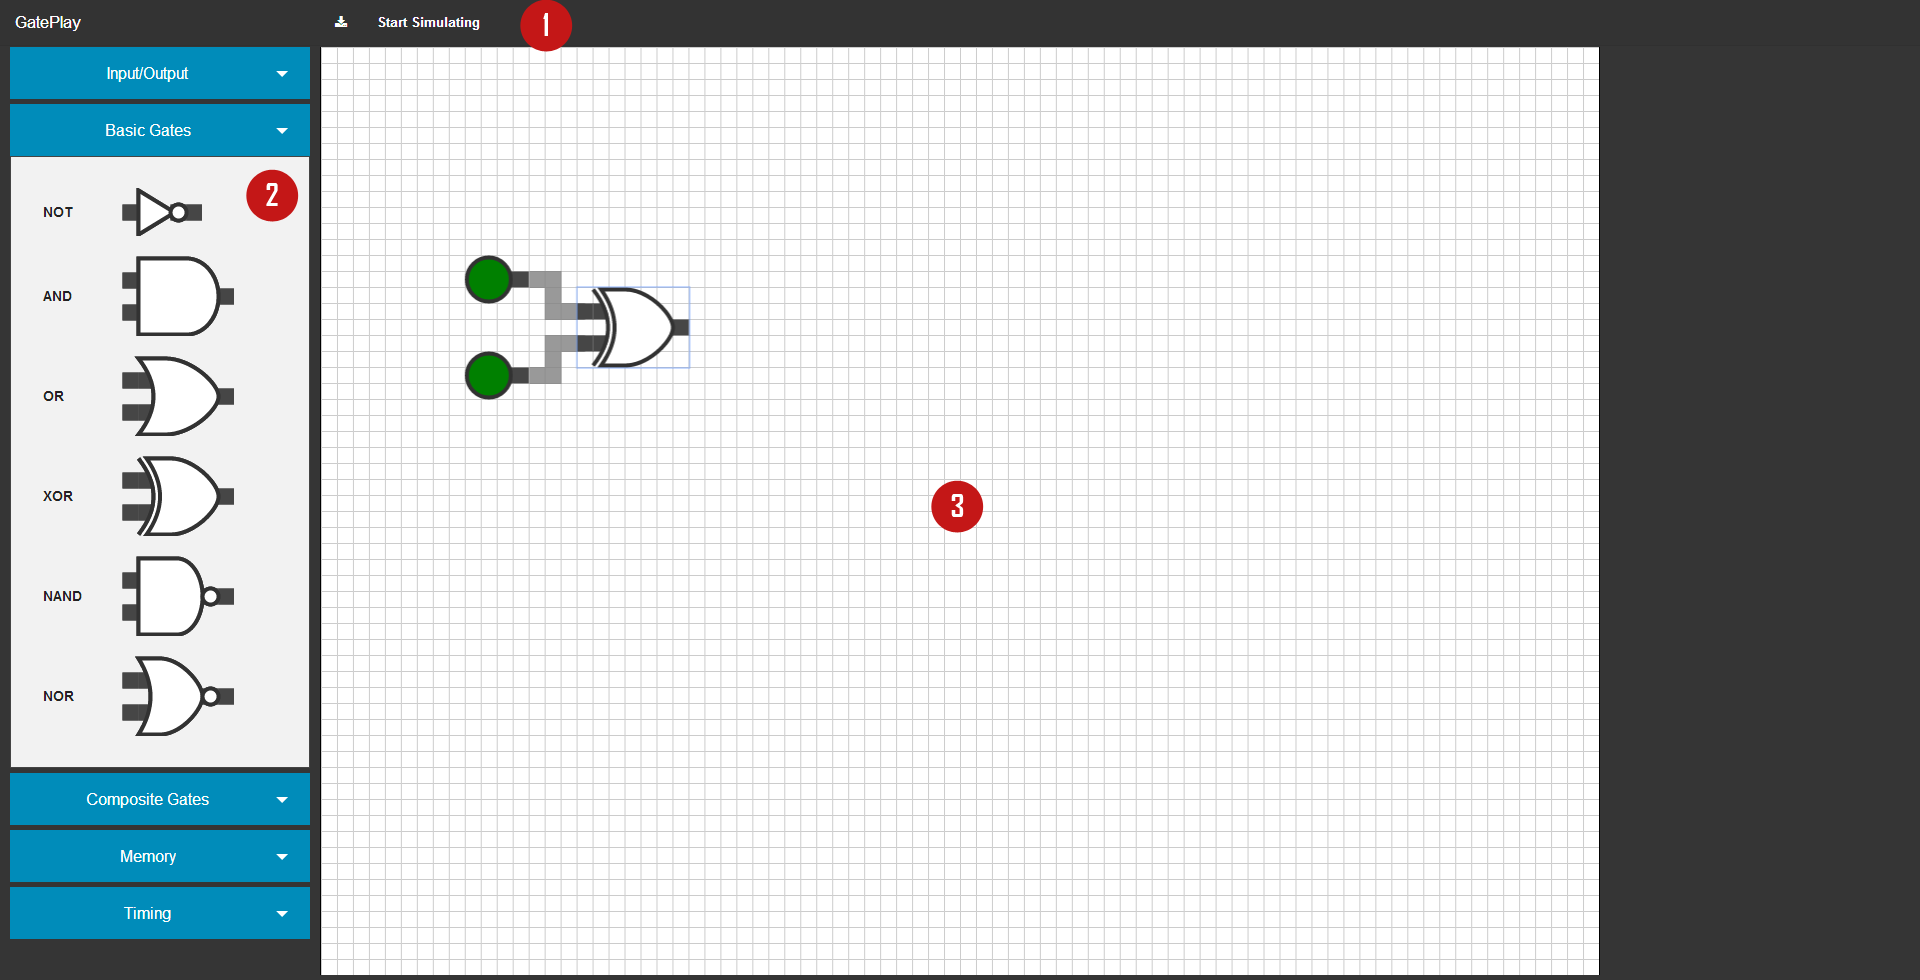
\includegraphics[width=\textheight,angle=90]{labelled.png}
    \caption{Drawing a circuit}
    \label{fig:interface}
\end{figure}

\begin{figure}[p]
    \centering
    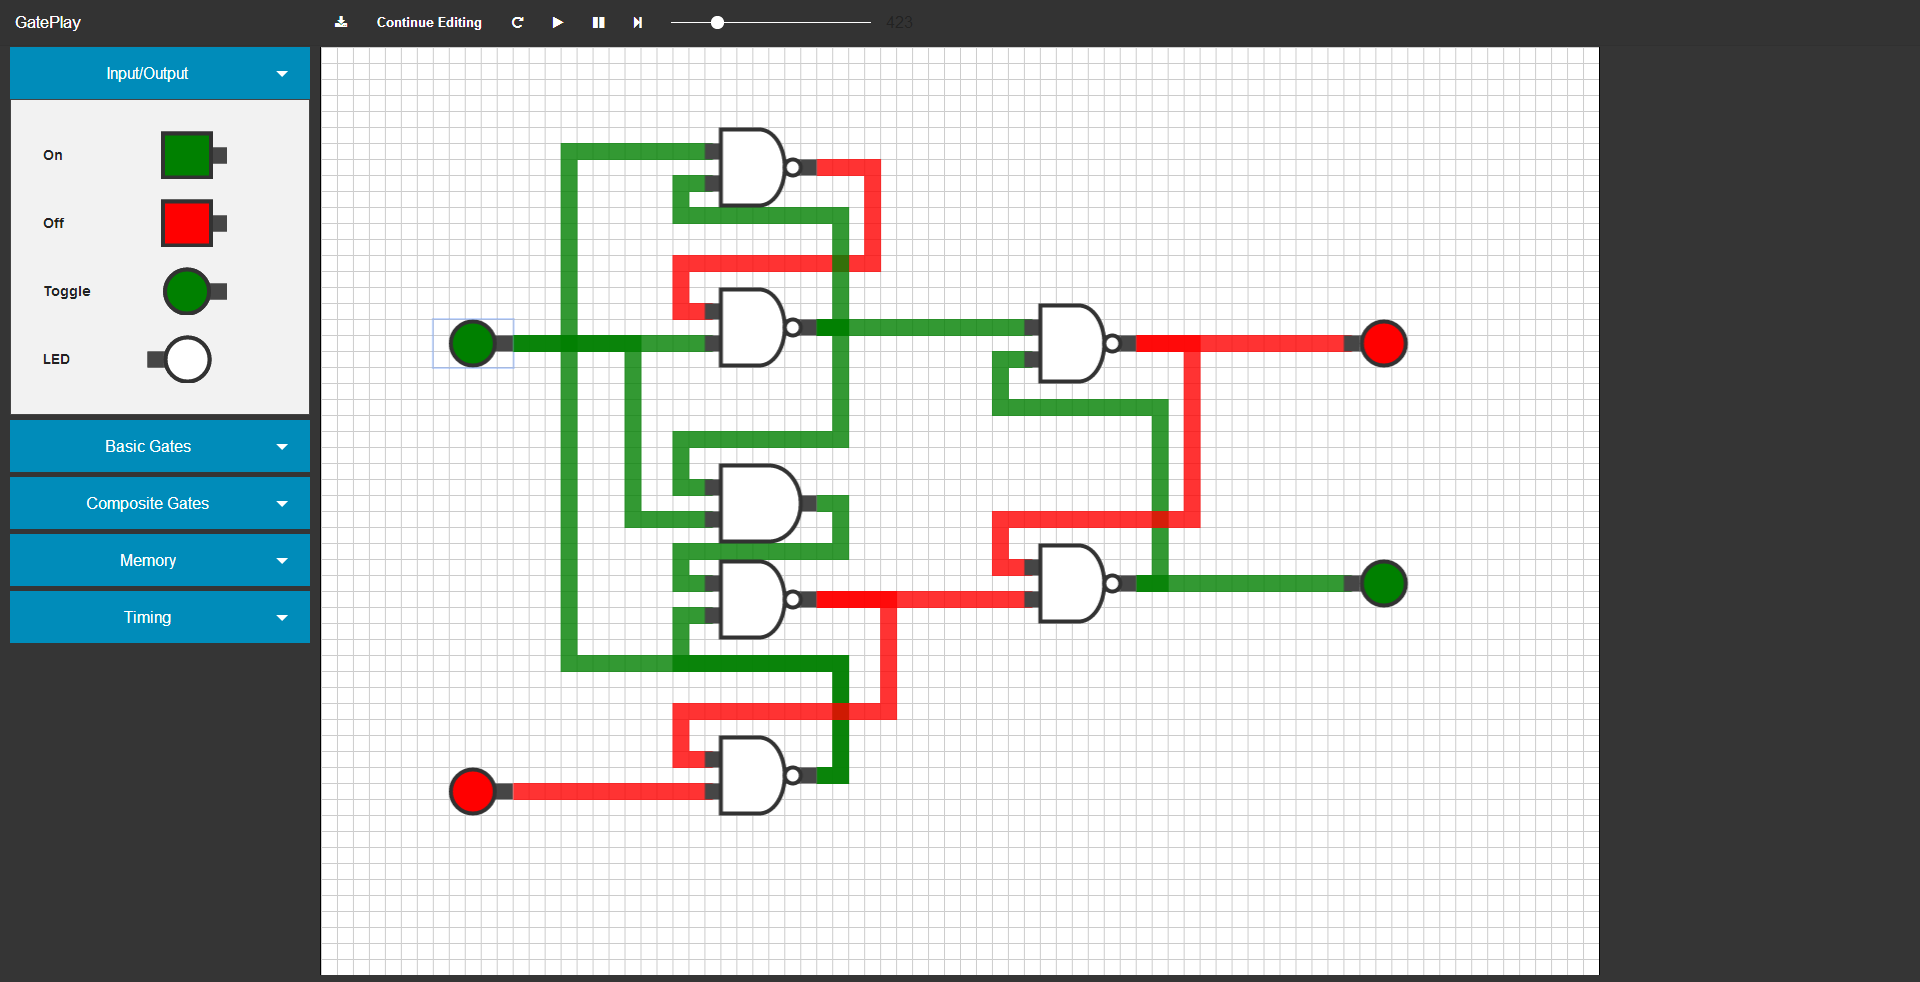
\includegraphics[width=\textheight,angle=90]{dflipflop.png}
    \caption{Simulating a D flip-flop}
    \label{fig:dflopflop}
\end{figure}